\section{Resolution Limits (Arithmetic Roots of Heisenberg's Uncertainty)}

\textit{(Resolution Limits - Arithmetic Roots of Heisenberg's Uncertainty)}

\begin{figure}[h]
\centering
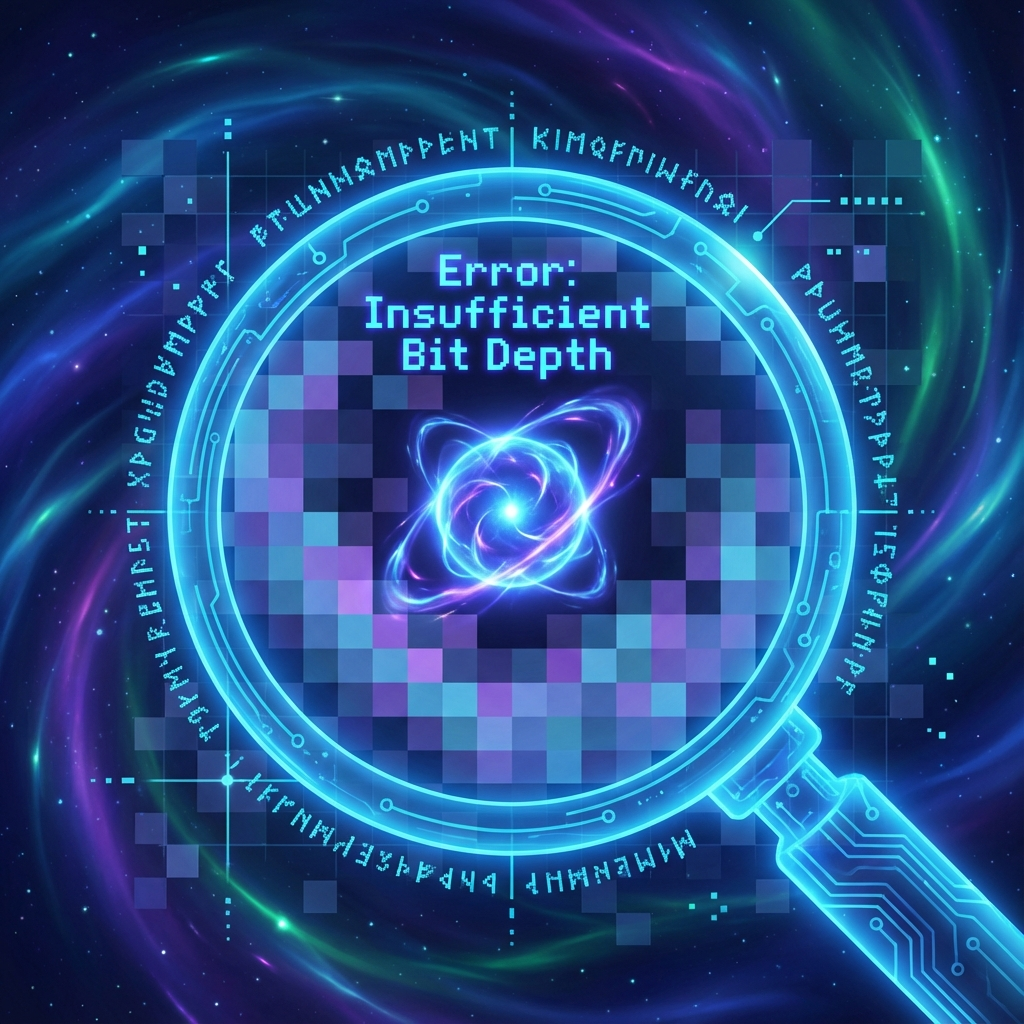
\includegraphics[width=0.8\textwidth]{assets/images/chapter06/heisenberg-pixelation.png}
\caption{Heisenberg Uncertainty: Resolution Limit}
\end{figure}

\begin{quote}
\textbf{``God doesn't play dice, but he does use finite-precision floating-point numbers. The uncertainty principle is not mysterious magic; it's a blurry jpg image. When you zoom to pixel level, you naturally can't see details; this is the iron law of any discrete system.''}
\end{quote}

In the first two volumes, we discussed macroscopic servers and networks. Now, we zoom in to see Azeroth's microscopic pixels---\textbf{quantum mechanics}.

Quantum mechanics' core feature is \textbf{Heisenberg's uncertainty principle}: You cannot simultaneously know a particle's position and velocity precisely.
In \textbf{Code of Azeroth} theory, this is neither perturbation nor ignorance. It's a mathematical corollary of the \textbf{Axiom of Finite Information}. Simply put, it's \textbf{insufficient resolution}.

\subsection{Video Memory Can't Store Infinite Decimals}

In classical mechanics, position is a real number. If you want to precisely write down a coordinate (like $\pi$), you need an infinitely long strip of paper.
But as we said in Chapter 1, the Titans' server has \textbf{finite bits}.

This means the system cannot store infinite-precision decimals. For any attribute, the system can only allocate finite \textbf{bit depth}.

Suppose the system allocates $N$ bits total to describe a particle.
\begin{itemize}
\item If you use many bits to describe \textbf{position} (very precise position), then fewer bits remain to describe \textbf{velocity} (blurry velocity).
\item Vice versa.
\end{itemize}

\textbf{Formula}:
\[
\text{position precision} + \text{velocity precision} \le \text{total memory}
\]

This is why when you measure position more precisely ($\Delta x \to 0$), momentum becomes more chaotic ($\Delta p \to \infty$). The system isn't unwilling to tell you; it's \textbf{because memory overflow, trailing digits are truncated}.

\subsection{Fourier Transform: The Seesaw of Time Domain and Frequency Domain}

This mathematically corresponds to \textbf{discrete Fourier transform}.

\begin{itemize}
\item \textbf{Position} is like \textbf{time domain} signal (which frame you appear in).
\item \textbf{Momentum} is like \textbf{frequency domain} signal (what's your frequency).
\end{itemize}

Mathematically, there's a dead law: You cannot create a signal that's both extremely short at this moment (position determined) and extremely narrow in spectrum (momentum determined).

\[
\Delta x \cdot \Delta p \ge \frac{\text{minimum pixel}}{2}
\]

This is purely an arithmetic fact. Like you cannot zoom an image to 1x1 pixel while retaining all details.

\subsection{Non-Commuting Operators: Data Type Conflicts}

In programmer's eyes, this uncertainty is due to \textbf{data type conversion}.

\begin{itemize}
\item \textbf{Measuring position}: Equivalent to executing \texttt{Read\_Position()}. System converts data to ``bitmap format.''
\item \textbf{Measuring momentum}: Equivalent to executing \texttt{Read\_Momentum()}. System converts data to ``spectrum format.''
\end{itemize}

These two operations are \textbf{mutually exclusive}. You cannot make a file both .bmp and .mp3. In this conversion process, information reorganization is inevitable.

\textbf{Theorem 6.1.1 (Mutually Exclusive Precision Protocol)}

Conjugate variables (position and momentum) are actually projections of the same underlying data in two different \textbf{views}. Since underlying data is only one copy, the system prohibits simultaneously opening two high-definition views.

\subsection{Lazy Evaluation and LOD Technology}

Finally, we connect the uncertainty principle with \textbf{Level of Detail (LOD)} technology.

In games, when the camera is far away, models are rough (low-poly). Only when you get very close does the graphics card load high-definition textures.

Heisenberg's principle is actually the universe rendering engine's \textbf{LOD switching mechanism}.

When an observer tries to ``see'' a particle with extremely high energy (short wavelength), they're actually forcing the system to perform \textbf{sub-pixel sampling}.
\begin{itemize}
\item To satisfy this excessive demand, the system must call extremely high-frequency data.
\item These high-frequency data correspond to huge momentum disturbances.
\item This disturbance is not ``measurement destroying the particle,'' but \textbf{high-frequency noise that the rendering engine must inject to generate high-precision coordinates}.
\end{itemize}

\textbf{Conclusion}:

Heisenberg's uncertainty principle is the \textbf{bandwidth theorem of discrete signal processing}. It protects the universe computer, preventing you from draining server memory through infinite-precision measurements. It's the \textbf{overflow protection} mechanism in physical laws.
